\chapter{Use Case Analysis}
\label{ch:use-case}
\newpage

This chapter presents the functional interactions between the external actors and the NewsPulse platform. The system boundary, actor roles, and use case relationships are modeled to illustrate how the microservices coordinate authentication, background news ingestion, multi-signal credibility evaluation, political bias detection, and counter-argument generation. Each use case is supported by a detailed specification table that defines preconditions, execution flows, and fallback behaviors.

\section{Use Case Model}
This section describes the system boundary and the three primary actors that interact with the NewsPulse platform.

As shown in Figure~\ref{fig:use_case_main}, the architecture coordinates interactions among three primary actors:
\begin{itemize}
    \item \textbf{News Service Provider (External API):} A secondary actor representing the external news aggregation layers (NewsAPI, NewsData.io, and GNews) and RSS feeds. This actor interacts strictly with the automated background collection routines of the system.
    \item \textbf{End User (Client):} The primary human actor who interacts with the React client interface. The user must authenticate to access the natural language processing endpoints. Once authorized, the user can trigger background news feeds, run analysis on articles or URLs, and save analyzed reports.
    \item \textbf{System Administrator (Admin):} The operations actor who monitors container health, evaluates request latency histograms, and reviews Redis and SQLite memory constraints via the Grafana and Prometheus dashboards.
\end{itemize}

\begin{figure}[h]
    \centering
    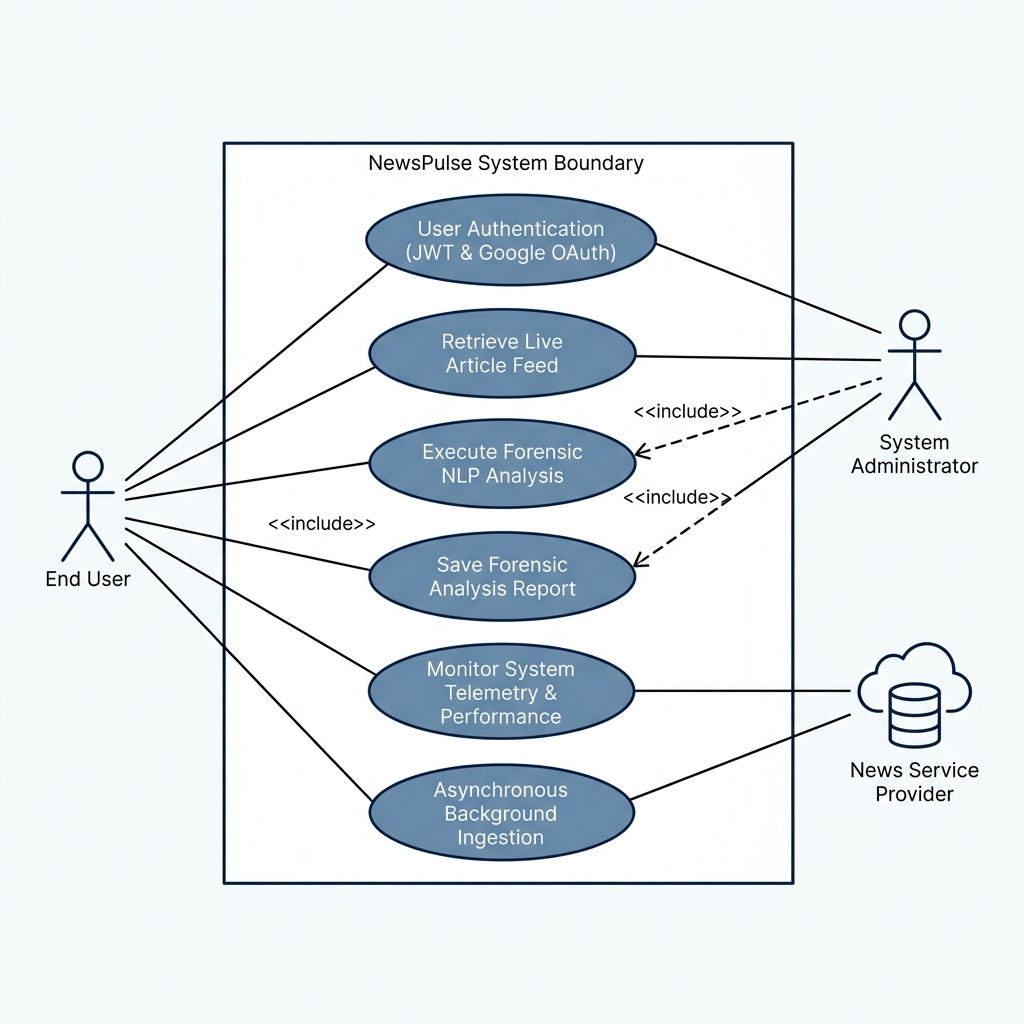
\includegraphics[width=0.85\linewidth]{BS_FYP_Figs/use_case_diagram.png}
    \caption{NewsPulse Decoupled System Use Case Diagram}
    \label{fig:use_case_main}
\end{figure}

The system boundary is governed by the centralized FastAPI Gateway. All stateful user interactions, such as running article analysis or saving reports, carry an \texttt{$\langle\langle$include$\rangle\rangle$} dependency on the validation of a valid JSON Web Token (JWT). Administrative telemetry operates in an isolated monitoring pipeline that does not expose secure user data.

\section{Use Cases Description}
This section describes the primary functional use cases of the NewsPulse microservices ecosystem. Each use case defines the actor, operational preconditions, the basic execution sequence, alternate flows for error and edge conditions, and the resulting post condition.

\subsection{User Registration and Authentication}
This use case manages user registration and authentication through the centralized \texttt{auth\_service}, verifying standard credentials or third-party Google OAuth tokens.

\begin{table}[h!]
    \begin{tabularx}{\textwidth}{|l|X|}
        \hline
        Title & Allow user to authenticate via standard credentials or third-party OAuth \\
        \hline
        Requirement & User must supply a valid username and password, or a verified Google identity token \\
        \hline
        Rational & To verify user identity and issue a signed JSON Web Token (JWT) for accessing the NLP microservices \\
        \hline
        Restriction or Risk & Time-drift on virtual machines hosting the containers may invalidate tokens prematurely \\
        \hline
        Dependency & SQLite authentication database, local Redis cache, active network interface \\
        \hline
        Priority & High (Critical Security Path) \\
        \hline
    \end{tabularx}
    \caption{User Authentication Function}
    \label{tab:table_user_login_function}
\end{table}

\subsubsection{Use Case 01: Standard Login}
This use case describes the step-by-step execution flow when a user authenticates using standard credentials or Google OAuth via the NewsPulse client.
\begin{table}[H]
    \renewcommand{\arraystretch}{1.3}
    \begin{tabularx}{\textwidth}{| X |}
        \hline
        \textbf{Standard Login and Authentication} \\
        \hline
        \textbf{Actor:}
        \begin{itemize}
            \item End User
            \item Google Identity Provider (for OAuth flow)
        \end{itemize} \\
        \hline
        \textbf{Preconditions:}
        \begin{itemize}
            \item The API Gateway and the \texttt{auth\_service} container are online and reachable.
            \item The local SQLite authentication database is connected via the SQLAlchemy engine.
        \end{itemize} \\
        \hline
        \textbf{Basic Flow:}
        \begin{itemize}
            \item The user submits credentials (username and password) via the client interface.
            \item The client encrypts the credentials using AES-256-GCM, wraps the symmetric key using the gateway's RSA-2048 public key, and transmits the Base64-encoded bundle.
            \item The API Gateway decrypts the payload using its private RSA key and forwards the credentials to the \texttt{auth\_service}.
            \item The \texttt{auth\_service} hashes the input password using \texttt{bcrypt} and compares it against the stored database hash.
            \item Upon successful validation, the gateway issues a JWT signed with HS256 and returns it to the client.
        \end{itemize} \\
        \hline
        \textbf{Alternate Flows:}
        \begin{itemize}
            \item \textbf{Alternate Flow 01 (Google OAuth):} If the user selects Google OAuth, the client sends a Google identity token. The gateway verifies it with Google's APIs, applying a 10-second clock skew allowance.
            \item \textbf{Alternate Flow 02 (Invalid Credentials):} If password validation fails, the gateway returns HTTP 401 Unauthorized and logs the failed attempt.
        \end{itemize} \\
        \hline
        \textbf{Post Condition:}
        \begin{itemize}
            \item The user receives a valid JWT token, enabling authorization for all subsequent NLP requests.
        \end{itemize} \\
        \hline
    \end{tabularx}
    \caption{Login Use Case}
    \label{tab:login_use_case}
\end{table}

\clearpage
\subsection{Execute Article Analysis}
This use case defines the execution sequence when an authorized user submits a raw article text block or URL for multi-signal analysis across the local NLP pipelines.

\begin{table}[h!]
    \begin{tabularx}{\textwidth}{|l|X|}
        \hline
        Title & Execute Multi-Signal Article Analysis \\
        \hline
        Requirement & User must present a valid, unexpired JWT \\
        \hline
        Rational & To generate article summaries, evaluate fake news credibility, map political polarization, and generate counter-arguments using local models \\
        \hline
        Restriction or Risk & Long-form text payloads may cause memory exhaustion and out-of-memory errors on standard CPUs \\
        \hline
        Dependency & Decoupled NLP microservices, Redis caching layer, isolated SQLite databases \\
        \hline
        Priority & High (Core Analysis Path) \\
        \hline
    \end{tabularx}
    \caption{Article Analysis Function}
    \label{tab:table_article_analysis_function}
\end{table}

\subsubsection{Use Case 02: Perform Article Inference}
This use case describes how the gateway coordinates the four parallel NLP containers to produce a complete forensic analysis of a submitted article.
\begin{table}[H]
    \renewcommand{\arraystretch}{1.3}
    \begin{tabularx}{\textwidth}{| X |}
        \hline
        \textbf{Multi-Signal NLP Article Inference} \\
        \hline
        \textbf{Actor:}
        \begin{itemize}
            \item Authenticated End User
        \end{itemize} \\
        \hline
        \textbf{Preconditions:}
        \begin{itemize}
            \item The user's JWT is verified by the gateway.
            \item The Summarizer, Fake News Detection, Political Bias, and Counter-Argument containers are online.
            \item The Redis cache container is active and reachable via the internal bridge network.
        \end{itemize} \\
        \hline
        \textbf{Basic Flow:}
        \begin{itemize}
            \item The user submits an article URL or text via the client interface.
            \item The client encrypts the request payload using AES-256-GCM and transmits it to the API Gateway.
            \item The gateway decrypts the payload, validates the JWT, and hashes the input text using SHA-256 to check the Redis cache.
            \item On a cache hit, the gateway returns the cached result immediately, bypassing the NLP models.
            \item On a cache miss, the gateway forwards the request in parallel to four NLP containers: Summarization (DistilBART-CNN-12-6), Fake News Detection (Sentinel BERT engine), Political Bias (DistilRoBERTa with windowed pooling), and Counter-Argument Engine (quantized Seq2Seq model).
            \item The gateway aggregates all outputs, writes the combined result to Redis, and returns the full analysis to the client.
        \end{itemize} \\
        \hline
        \textbf{Alternate Flows:}
        \begin{itemize}
            \item \textbf{Alternate Flow 01 (Input Truncation):} If the input text exceeds 2500 characters, the summarizer truncates the text to protect system memory.
            \item \textbf{Alternate Flow 02 (Heuristic Fallbacks):} If the DistilBART summarizer fails, a term-frequency sentence extraction algorithm is used. If the counter-argument engine fails, a template-based response is returned.
            \item \textbf{Alternate Flow 03 (Credibility Adjustments):} The credibility engine applies domain multipliers and caps objective styling scores at 0.49 to suppress false positive fake news classifications.
        \end{itemize} \\
        \hline
        \textbf{Post Condition:}
        \begin{itemize}
            \item The client receives the aggregated analysis, maps credibility and polarization using charts, and highlights the most sensational sentence using Explainable AI (XAI).
        \end{itemize} \\
        \hline
    \end{tabularx}
    \caption{Article Inference Use Case}
    \label{tab:article_inference_use_case}
\end{table}

\clearpage
\subsection{Manage Saved Articles}
This use case describes how an authenticated user persists a completed forensic analysis report to the local SQLite database for later retrieval.

\begin{table}[h!]
    \begin{tabularx}{\textwidth}{|l|X|}
        \hline
        Title & Save and Retrieve Forensic Analysis Report \\
        \hline
        Requirement & User must possess a validated, active JWT and a completed analysis \\
        \hline
        Rational & To allow users to store analyzed articles and access their history from the saved articles panel \\
        \hline
        Restriction or Risk & SQLite write locks under concurrent access may delay the save operation \\
        \hline
        Dependency & SQLite user database, SQLAlchemy ORM, active JWT session \\
        \hline
        Priority & Medium (User Persistence Path) \\
        \hline
    \end{tabularx}
    \caption{Manage Saved Articles Function}
    \label{tab:table_save_article_function}
\end{table}

\subsubsection{Use Case 03: Manage Saved Articles}
This use case describes the steps taken when a user saves a completed analysis report to their personal dashboard.
\begin{table}[H]
    \renewcommand{\arraystretch}{1.3}
    \begin{tabularx}{\textwidth}{| X |}
        \hline
        \textbf{Save Forensic Analysis Report} \\
        \hline
        \textbf{Actor:}
        \begin{itemize}
            \item Authenticated End User
        \end{itemize} \\
        \hline
        \textbf{Preconditions:}
        \begin{itemize}
            \item The user possesses a validated, active JWT.
            \item The forensic analysis for the target article has successfully completed.
        \end{itemize} \\
        \hline
        \textbf{Basic Flow:}
        \begin{itemize}
            \item The user selects the Save Article option on the client dashboard.
            \item The client encrypts the request and transmits it to the API Gateway.
            \item The gateway validates the JWT and forwards the payload to the user service.
            \item The user service connects to the SQLite database via SQLAlchemy and writes the analysis records to the saved articles table.
            \item The database confirms the write and the gateway returns HTTP 201 Created to the client.
        \end{itemize} \\
        \hline
        \textbf{Alternate Flows:}
        \begin{itemize}
            \item \textbf{Alternate Flow 01 (Database Lock):} If the SQLite database is locked by another thread, the SQLAlchemy engine retries with a 5-second timeout before returning HTTP 500.
        \end{itemize} \\
        \hline
        \textbf{Post Condition:}
        \begin{itemize}
            \item The analysis report is securely stored and the user can retrieve it later from the saved articles panel.
        \end{itemize} \\
        \hline
    \end{tabularx}
    \caption{Save Article Use Case}
    \label{tab:save_article_use_case}
\end{table}

\clearpage
\subsection{Monitor System Telemetry}
This use case describes how the System Administrator accesses real-time performance metrics via the Prometheus and Grafana monitoring stack.

\begin{table}[h!]
    \begin{tabularx}{\textwidth}{|l|X|}
        \hline
        Title & Access Container and System Telemetry \\
        \hline
        Requirement & Prometheus and Grafana containers must be active in the Docker bridge network \\
        \hline
        Rational & To give the administrator visibility into request latencies, CPU load, and Redis cache performance \\
        \hline
        Restriction or Risk & If a backend container goes offline, Prometheus marks its target as DOWN \\
        \hline
        Dependency & Prometheus, Grafana, backend \texttt{/metrics} endpoints, Docker bridge network \\
        \hline
        Priority & Medium (Operational Monitoring Path) \\
        \hline
    \end{tabularx}
    \caption{Monitor System Telemetry Function}
    \label{tab:table_telemetry_function}
\end{table}

\subsubsection{Use Case 04: Monitor Telemetry Metrics}
This use case describes the steps taken by the System Administrator to access and review real-time system performance data.
\begin{table}[H]
    \renewcommand{\arraystretch}{1.3}
    \begin{tabularx}{\textwidth}{| X |}
        \hline
        \textbf{Access Container and System Telemetry} \\
        \hline
        \textbf{Actor:}
        \begin{itemize}
            \item System Administrator
        \end{itemize} \\
        \hline
        \textbf{Preconditions:}
        \begin{itemize}
            \item The Prometheus and Grafana containers are active in the Docker bridge network.
            \item All backend containers are exposing their \texttt{/metrics} endpoints.
        \end{itemize} \\
        \hline
        \textbf{Basic Flow:}
        \begin{itemize}
            \item The Administrator opens the Grafana monitoring dashboard via the configured local port.
            \item Grafana queries the Prometheus time-series database for aggregated system metrics.
            \item Prometheus scrapes the \texttt{/metrics} endpoints of all backend services and aggregates Gunicorn and Uvicorn worker statistics via the \texttt{MultiProcessCollector}.
            \item The Administrator reviews system health metrics including request latencies, CPU utilization, and Redis cache hit ratios.
        \end{itemize} \\
        \hline
        \textbf{Alternate Flows:}
        \begin{itemize}
            \item \textbf{Alternate Flow 01 (Service Unreachable):} If a service is offline, Prometheus marks its target status as DOWN and triggers an alert in the Grafana dashboard, notifying the Administrator to restart the container.
        \end{itemize} \\
        \hline
        \textbf{Post Condition:}
        \begin{itemize}
            \item The Administrator obtains real-time system performance insights to manage container capacity and service availability.
        \end{itemize} \\
        \hline
    \end{tabularx}
    \caption{Telemetry Monitoring Use Case}
    \label{tab:telemetry_use_case}
\end{table}
